\documentclass[12pt]{beamer}
\usepackage[english, russian]{babel}
\usepackage[utf8]{inputenc}
\usepackage{graphicx}
\usepackage{hyperref}
\usepackage{minted}

\hypersetup{
    colorlinks=true,
    linkcolor=blue,      
    urlcolor=cyan,
}

\graphicspath{ {./assets/} }

\usetheme{Madrid}

\title{Material Design}
\author{Karabalin Ruslan}
\date{21 декабря 2024 г.}

\begin{document}
	
	\begin{frame}
		\titlepage
	\end{frame}
	
    \begin{frame}
        \frametitle{Android 1.0 - 2.x}
        \begin{center}
            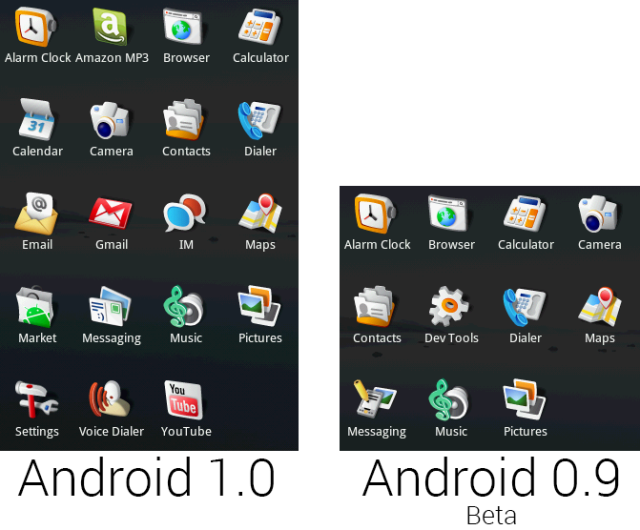
\includegraphics[width=0.7\textwidth]{android-1-0.png}
        \end{center}
    \end{frame}

    \begin{frame}
        \frametitle{Android Honeycomb}
        \begin{center}
            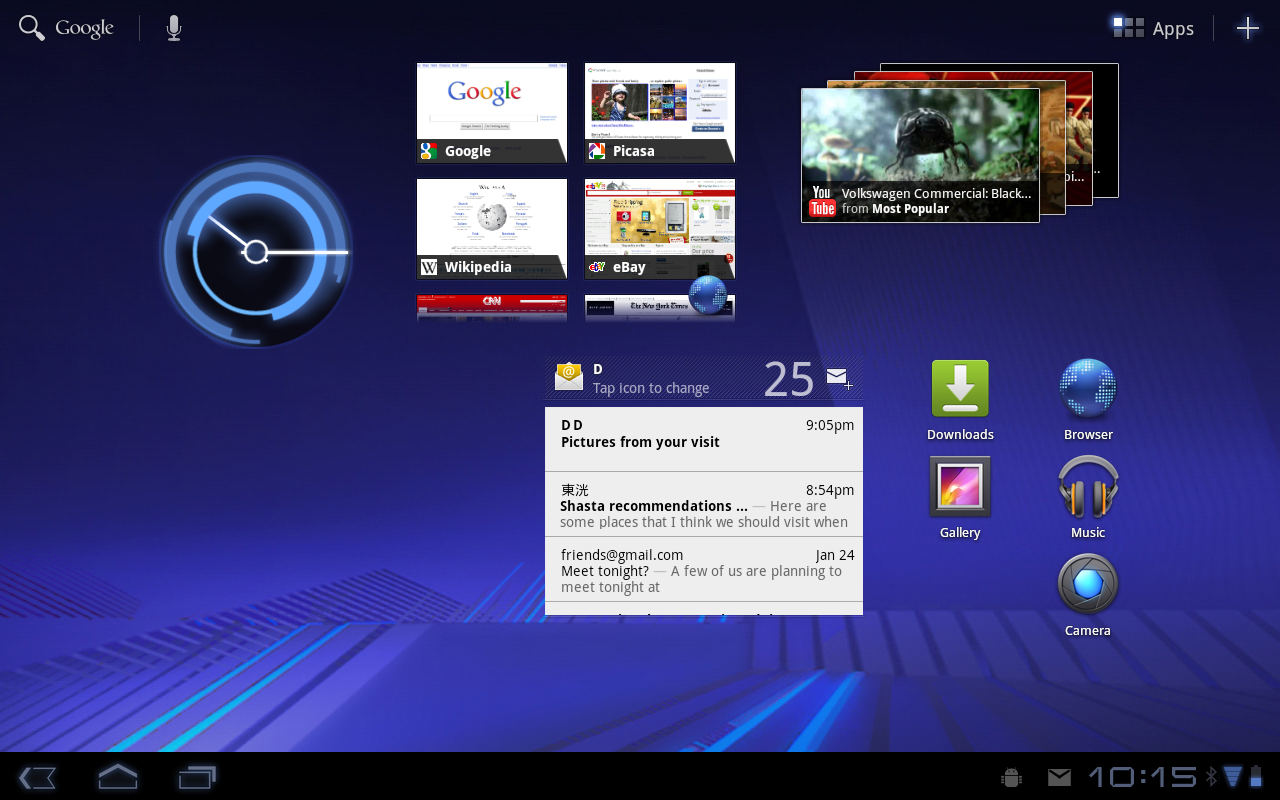
\includegraphics[width=0.9\textwidth]{android-3-0.png}
        \end{center}
    \end{frame}

    \begin{frame}
        \frametitle{Material Design 1}
        \begin{columns}
            \begin{column}{0.3\textwidth}
                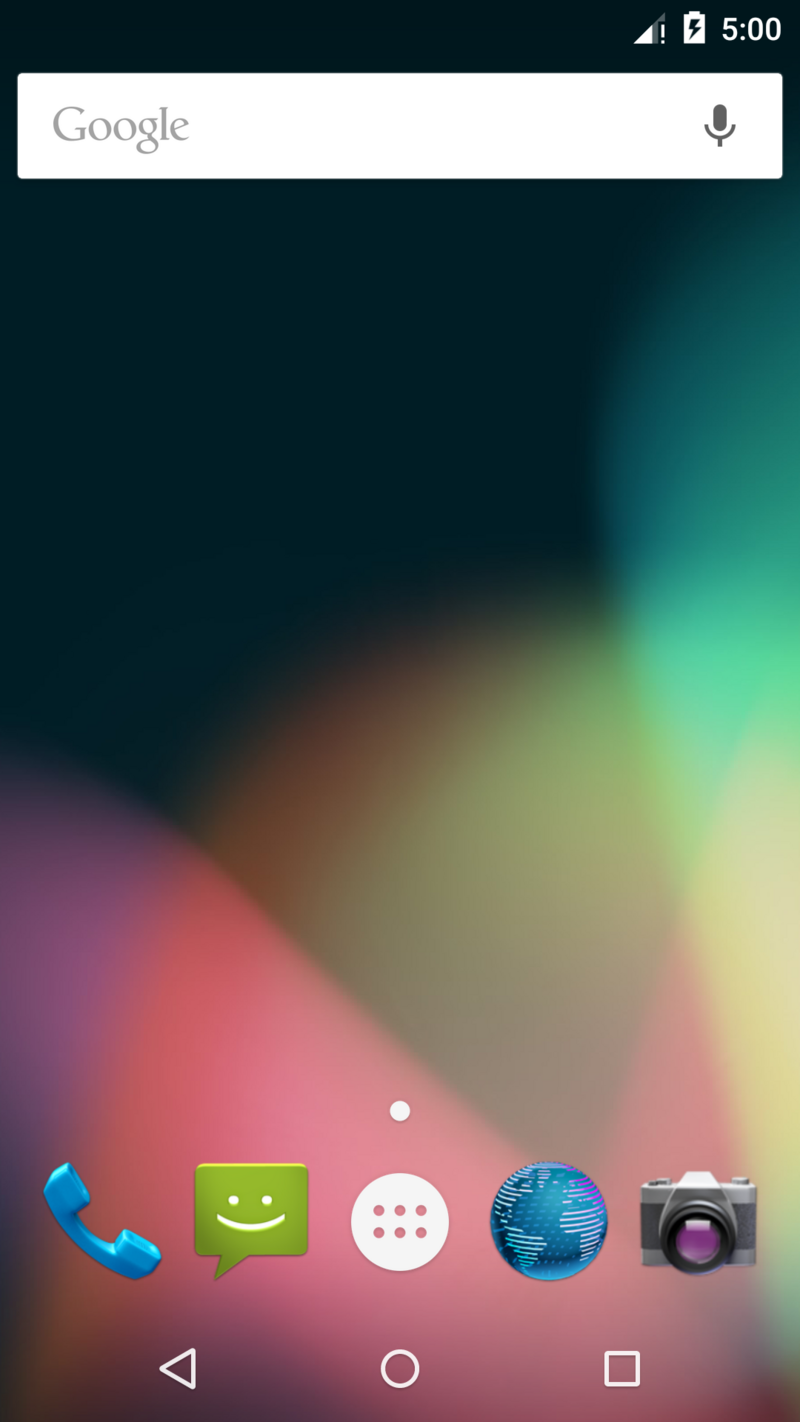
\includegraphics[width=0.7\textwidth]{android-5-0.png}
            \end{column}
            \begin{column}{0.3\textwidth}
                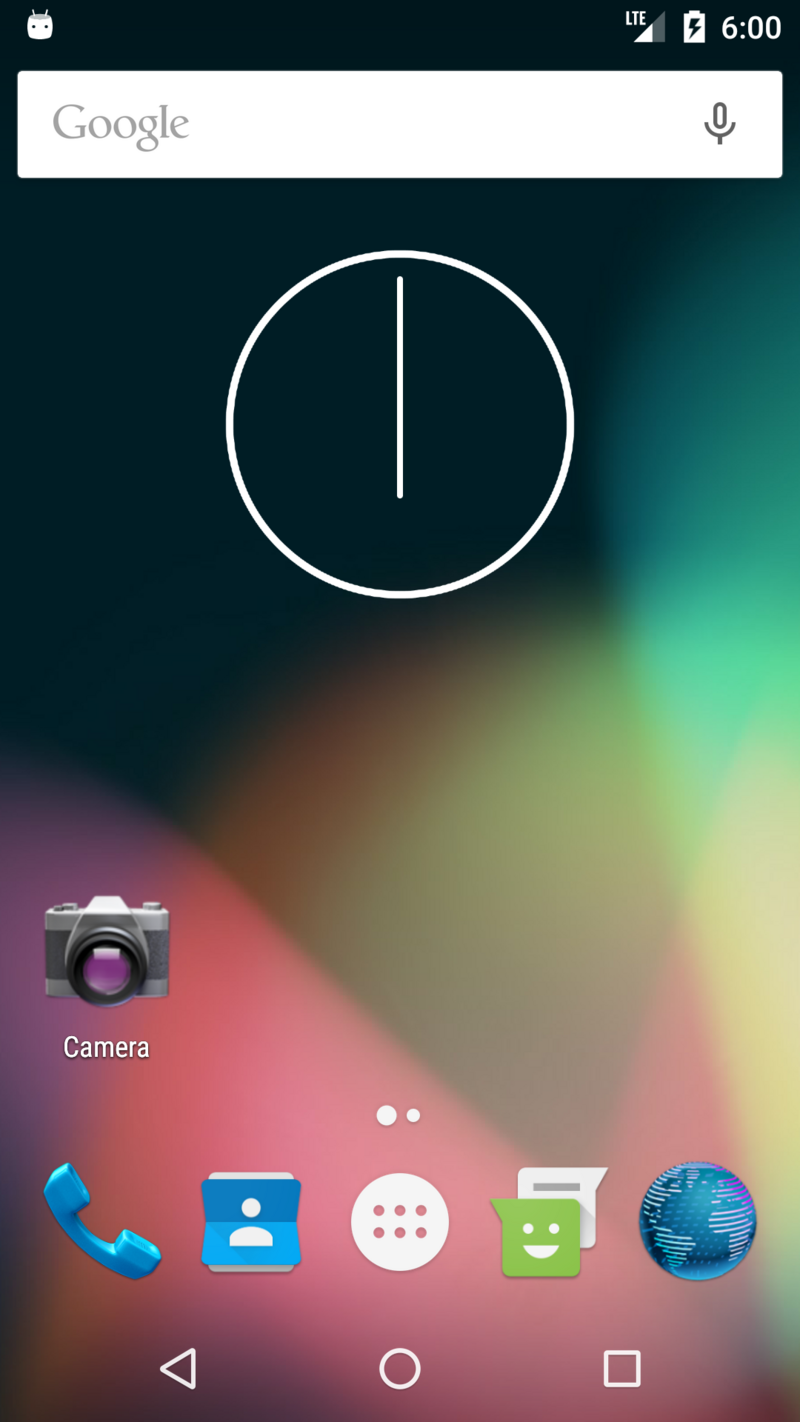
\includegraphics[width=0.7\textwidth]{android-6-0.png}
            \end{column}
            \begin{column}{0.3\textwidth}
                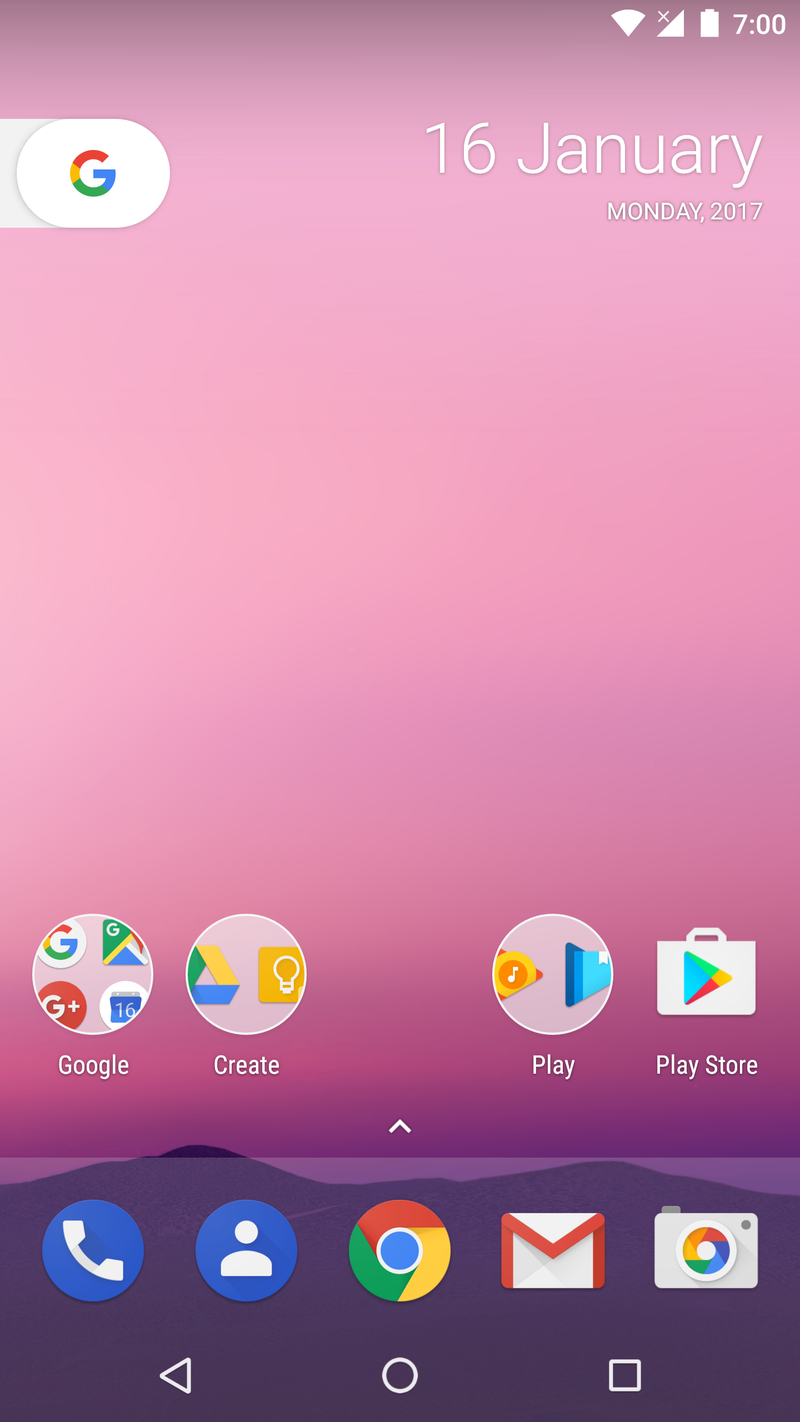
\includegraphics[width=0.7\textwidth]{android-7-0.png}
            \end{column}
        \end{columns}
    \end{frame}

	\begin{frame}
		\frametitle{What is Material?}
		\href{https://m3.material.io/}{Material Design}
        - это система дизайна от Google
        для создания интуитивно понятных,
        согласованных и визуально привлекательных приложений. \\
		
        Впервые представлен в 2014 году для
        улучшения пользовательского опыта на всех платформах. \\

        Основан на реальных свойствах материалов
        (например, бумаги и чернил). \\

		Последняя версия, Material 3,
        обеспечивает персональный, адаптивный
        и выразительный опыт - от динамических цветов
        и расширенной доступности до основ
        для макетов на больших экранах и дизайнерских решений.	
	\end{frame}
	
	\begin{frame}
		\frametitle{Main Goal}
        \begin{columns}
            \begin{column}{0.5\textwidth}
                \begin{itemize}
                    \item Обеспечение единого пользовательского опыта
                    на смартфонах, планшетах и компьютерах.
                    \item Имитация физики реального мира
                    (движение, глубина, тени).
                    \item Работает на любых экранах и разрешениях.
                    \item Включает читаемую типографику,
                    контрастность цветов и поддержку вспомогательных технологий. 
                \end{itemize}
            \end{column}
            \begin{column}{0.5\textwidth}
                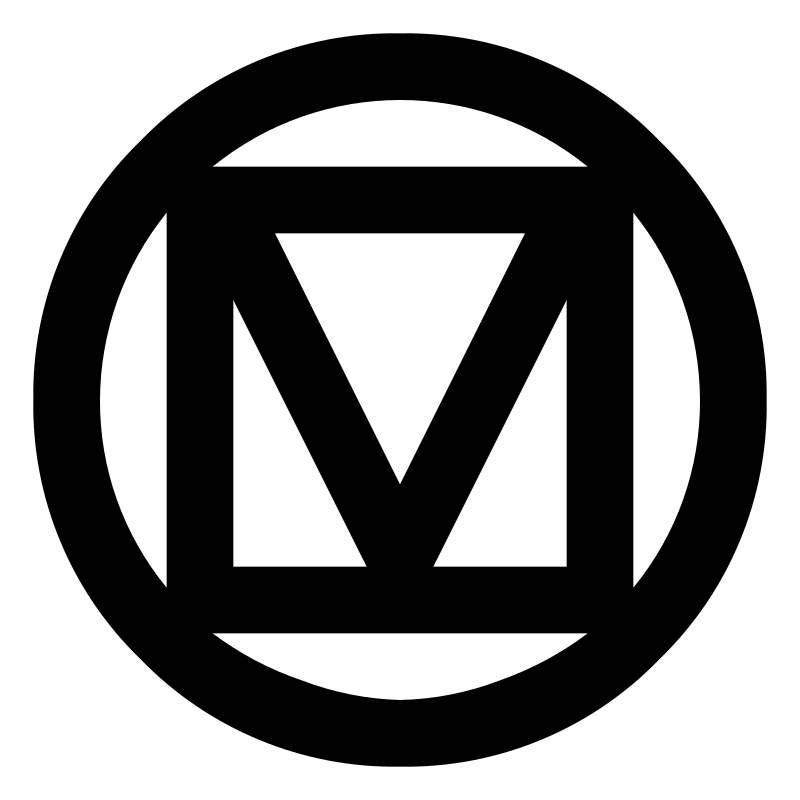
\includegraphics[width=0.8\textwidth]{md.png}
            \end{column}
        \end{columns}

	\end{frame}

    \begin{frame}
        \frametitle{Material Design 2}
        \begin{columns}
            \begin{column}{0.5\textwidth}
                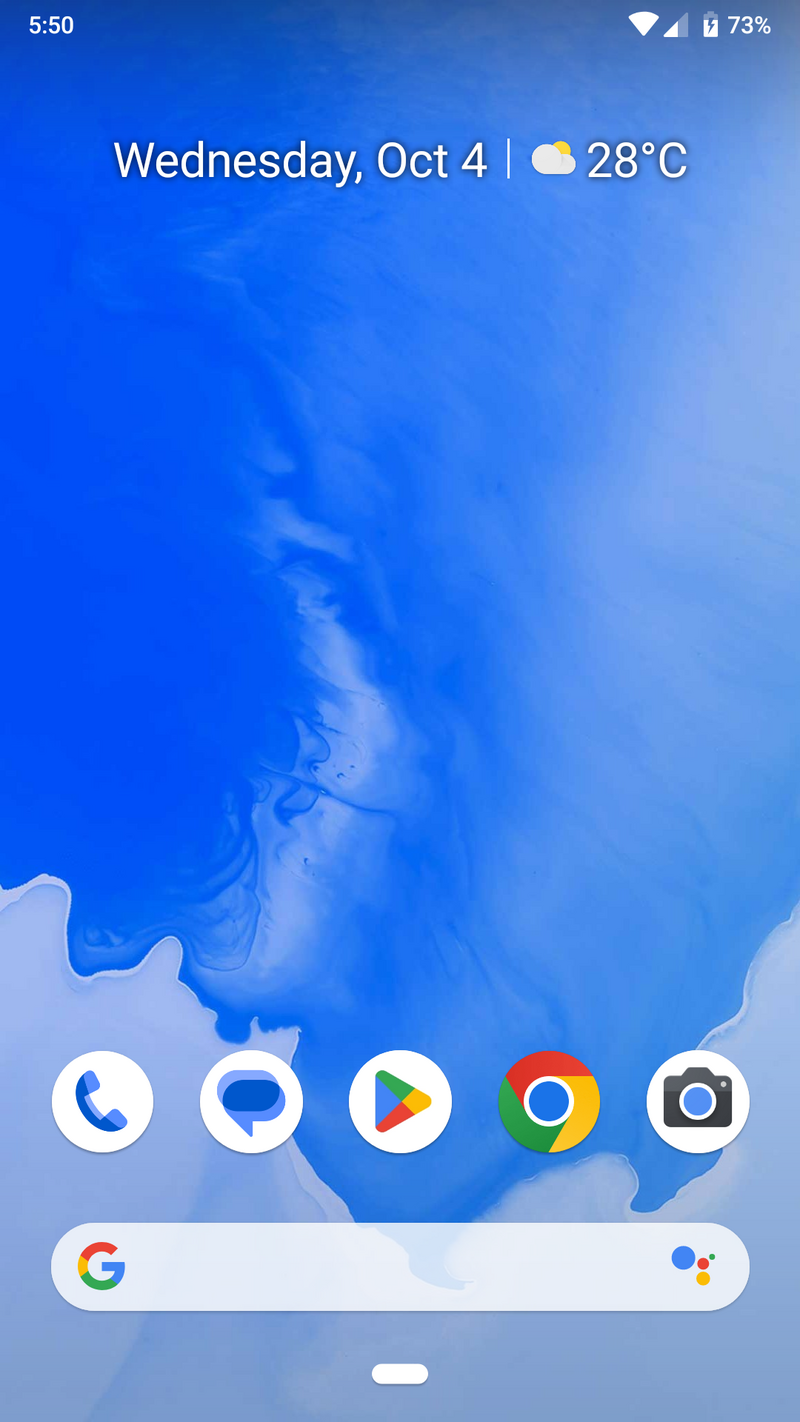
\includegraphics[width=0.7\textwidth]{android-9-0.png}
            \end{column}
            \begin{column}{0.5\textwidth}
                \begin{itemize}
                    \item Ввел концепцию Material Theming, которая позволяет разработчикам адаптировать дизайн под нужды бренда.
                    \item Полностью поддерживает темный режим.
                    \item Анимации стали более утонченными и выразительными.
                    \item Улучшенные цветовые контрасты для слабовидящих пользователей.
                \end{itemize}
            \end{column}
        \end{columns}
    \end{frame}

    \begin{frame}
        \frametitle{Material Design 3}
        \begin{columns}
            \begin{column}{0.5\textwidth}
                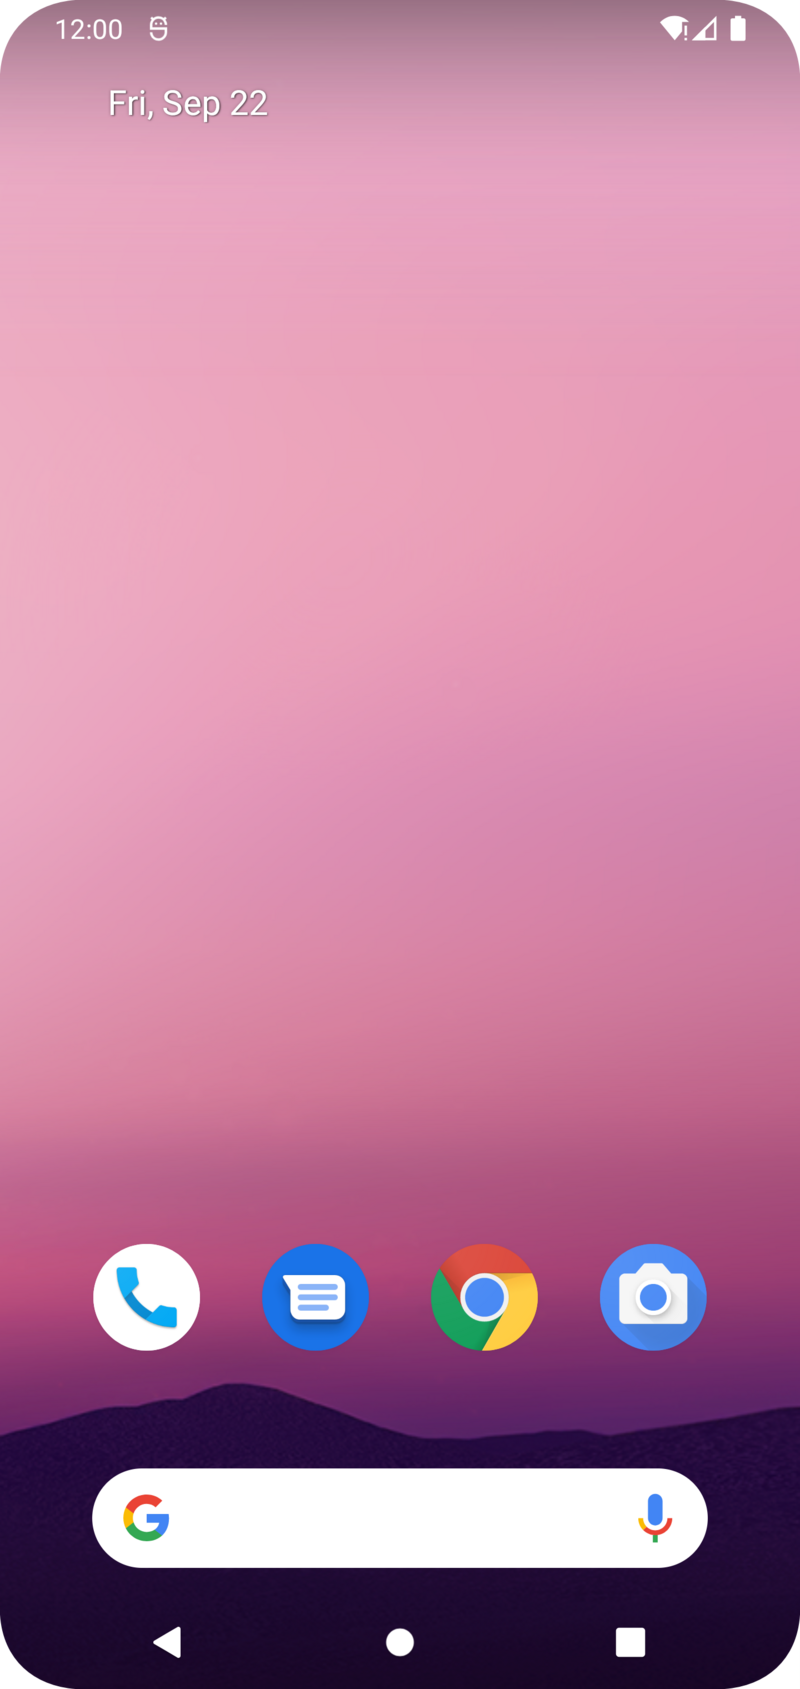
\includegraphics[width=0.6\textwidth]{android-12-0.png}
            \end{column}
            \begin{column}{0.5\textwidth}
                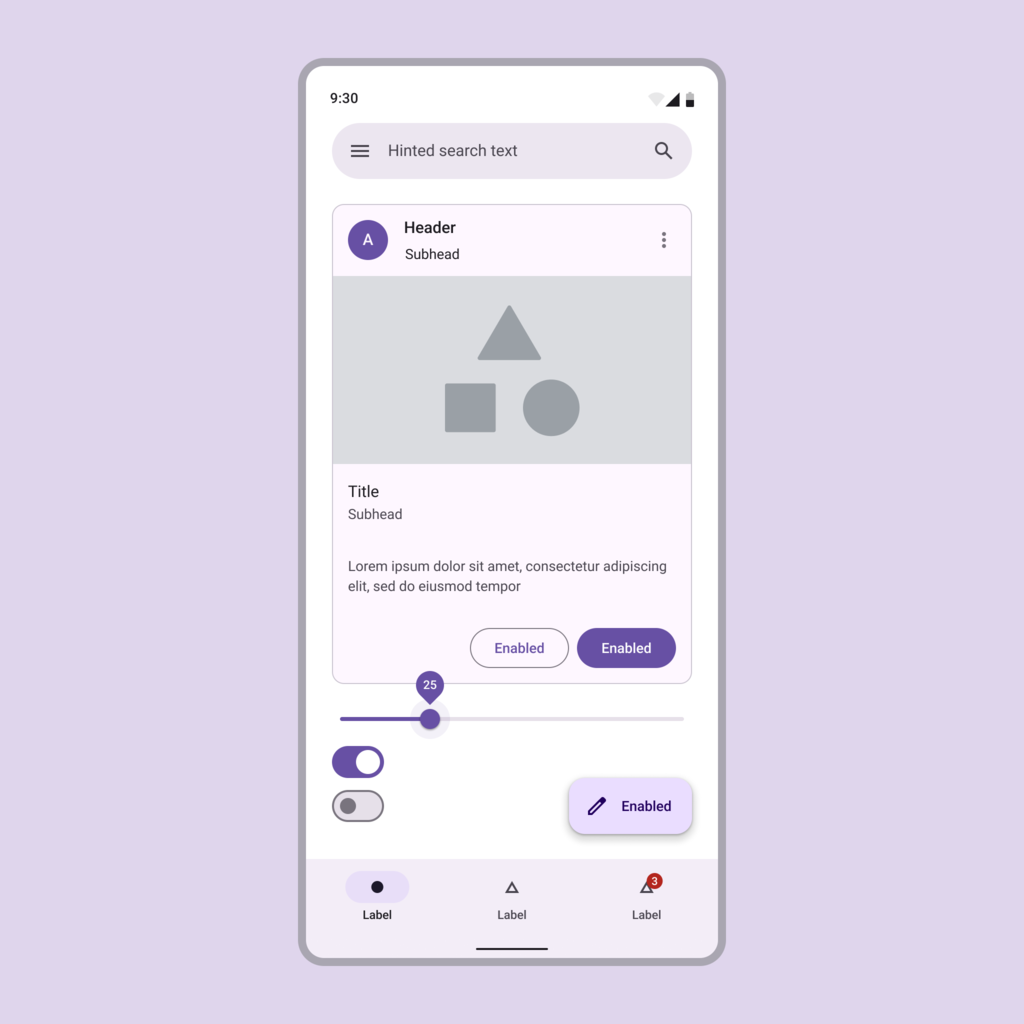
\includegraphics[width=1\textwidth]{md-3.png}
            \end{column}
        \end{columns}
    \end{frame}

    \begin{frame}
        \frametitle{Jetpack Compose}
        \begin{columns}
            \begin{column}{0.5\textwidth}
                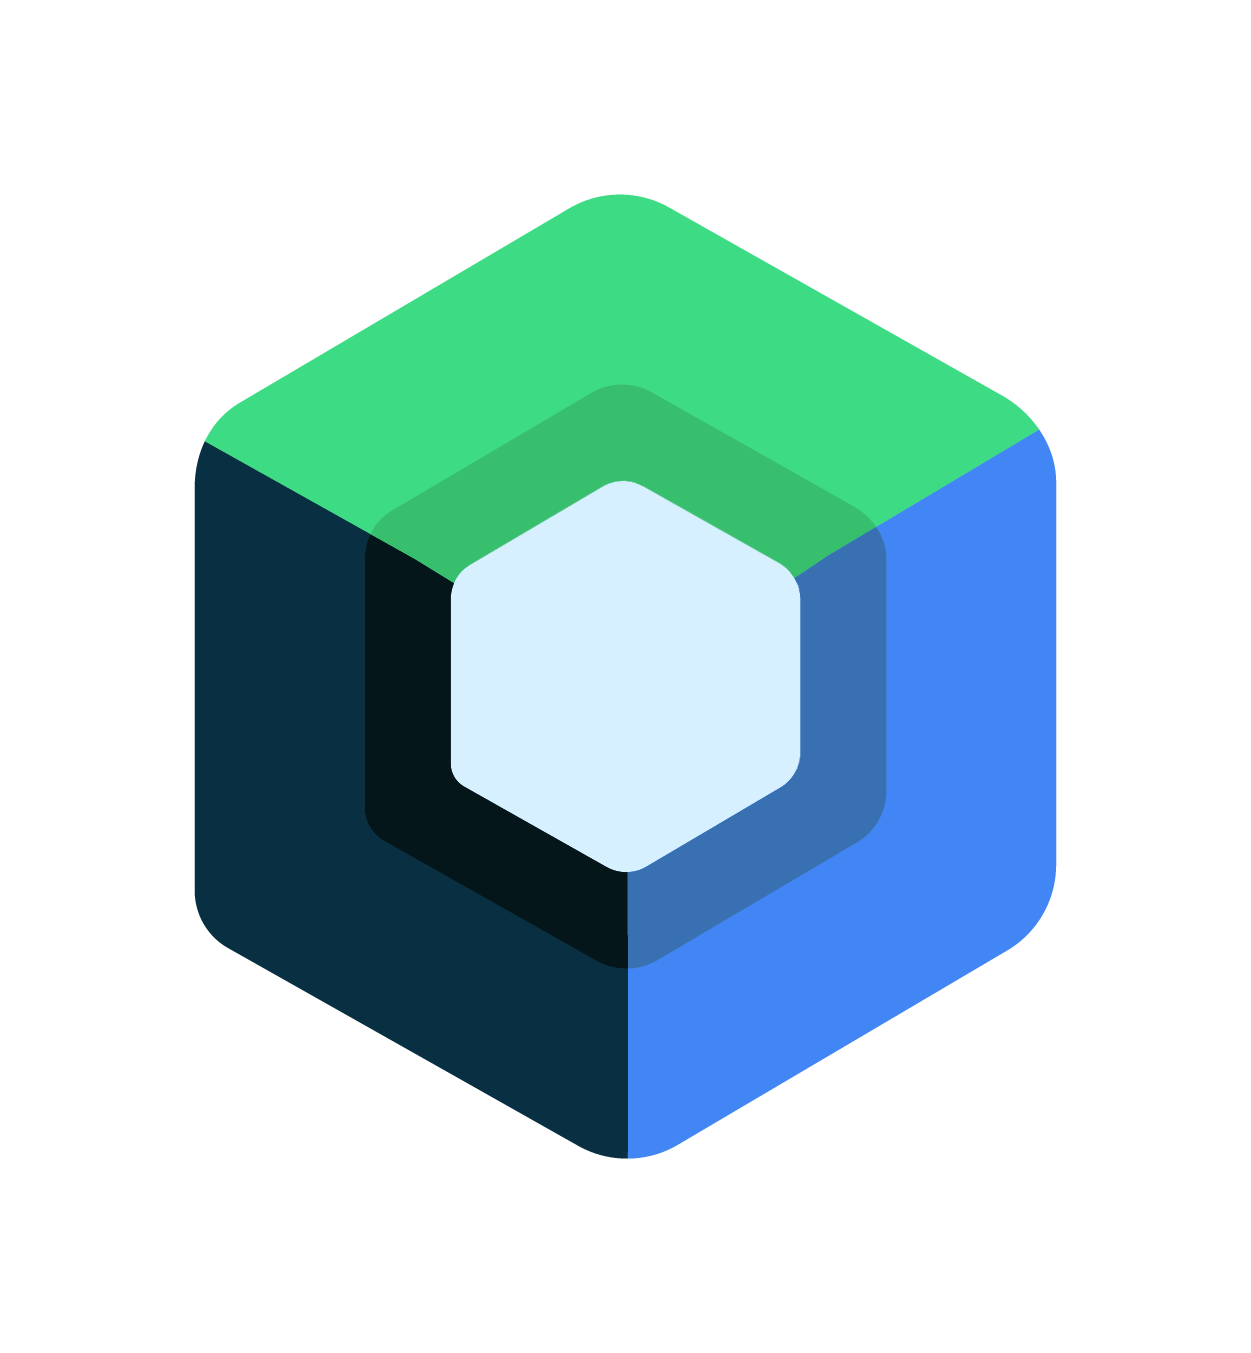
\includegraphics[width=0.8\textwidth]{jc.png}
            \end{column}

            \begin{column}{0.5\textwidth}
                \href{https://developer.android.com/compose}{Jetpack Compose}
                - это современный набор инструментов Android
                для создания нативного пользовательского интерфейса. \\

                Поддерживает Material Design 3 по-умолчанию.
            \end{column}
        \end{columns}
    \end{frame}

    \begin{frame}
        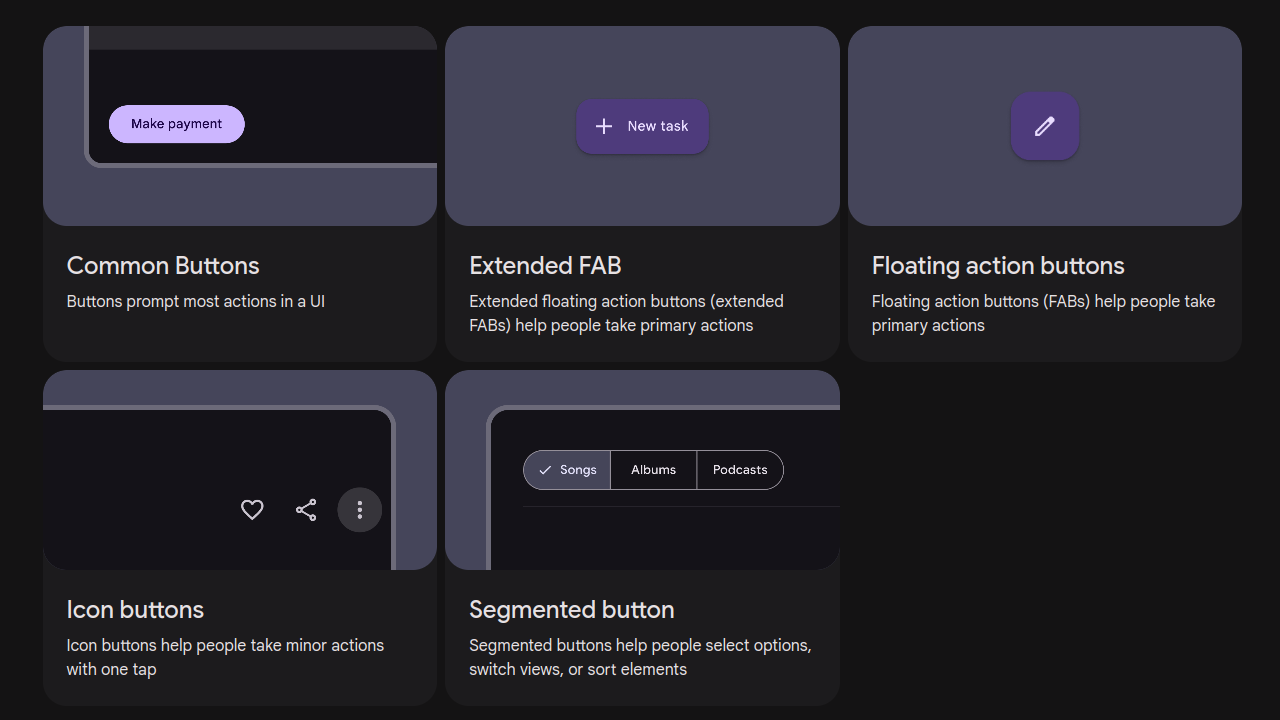
\includegraphics[width=1\textwidth]{actions.png}
    \end{frame}

    \begin{frame}
        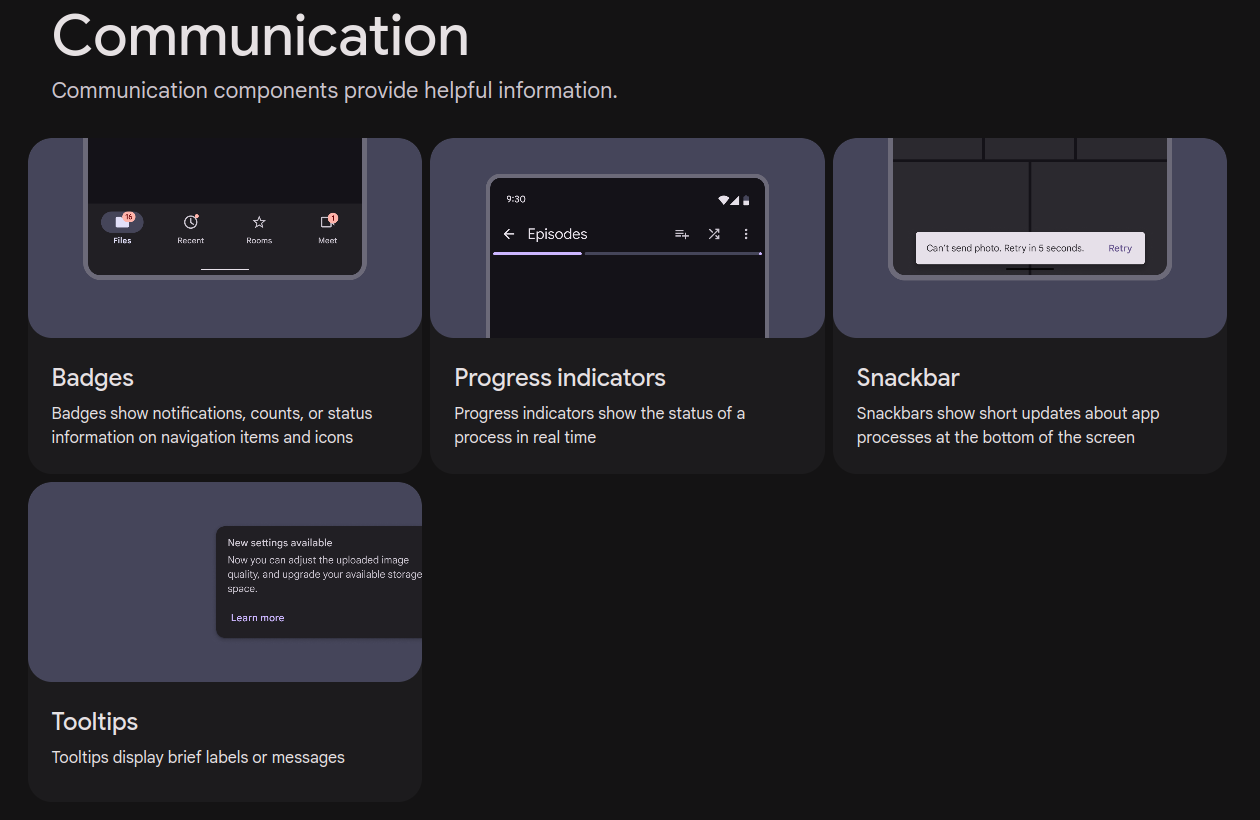
\includegraphics[width=1\textwidth]{communication.png}
    \end{frame}

    \begin{frame}
        \begin{center}
            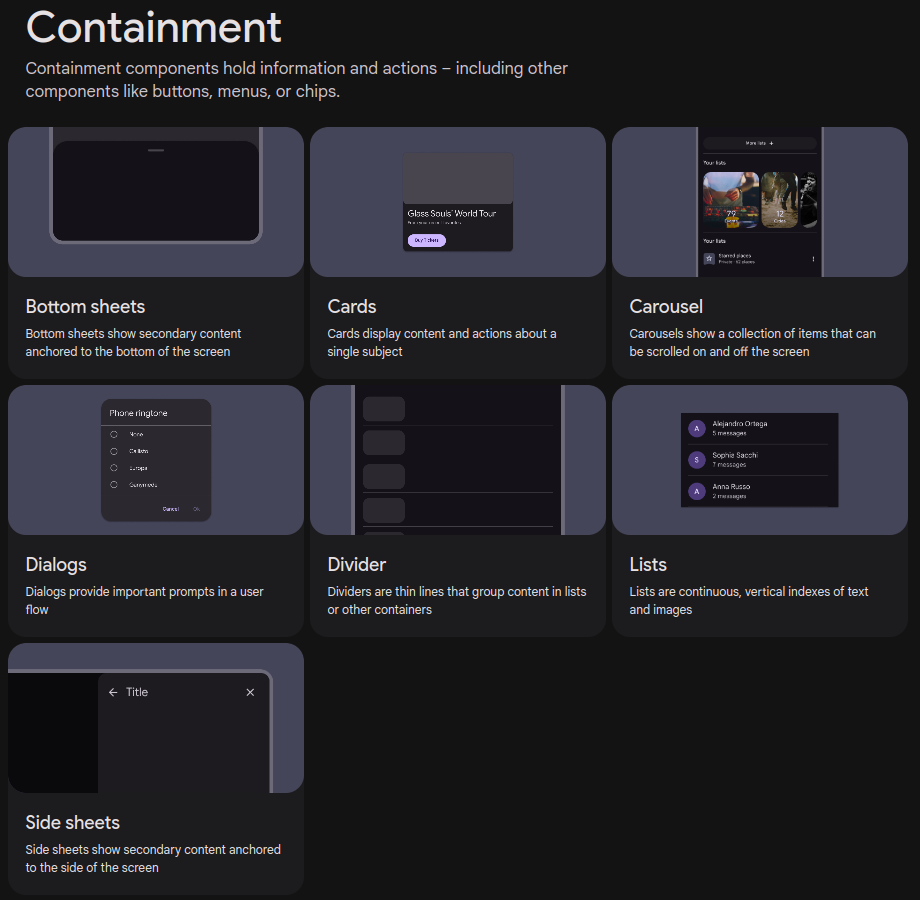
\includegraphics[width=0.7\textwidth]{containment.png}
        \end{center}
    \end{frame}

	\begin{frame}
        \begin{center}
            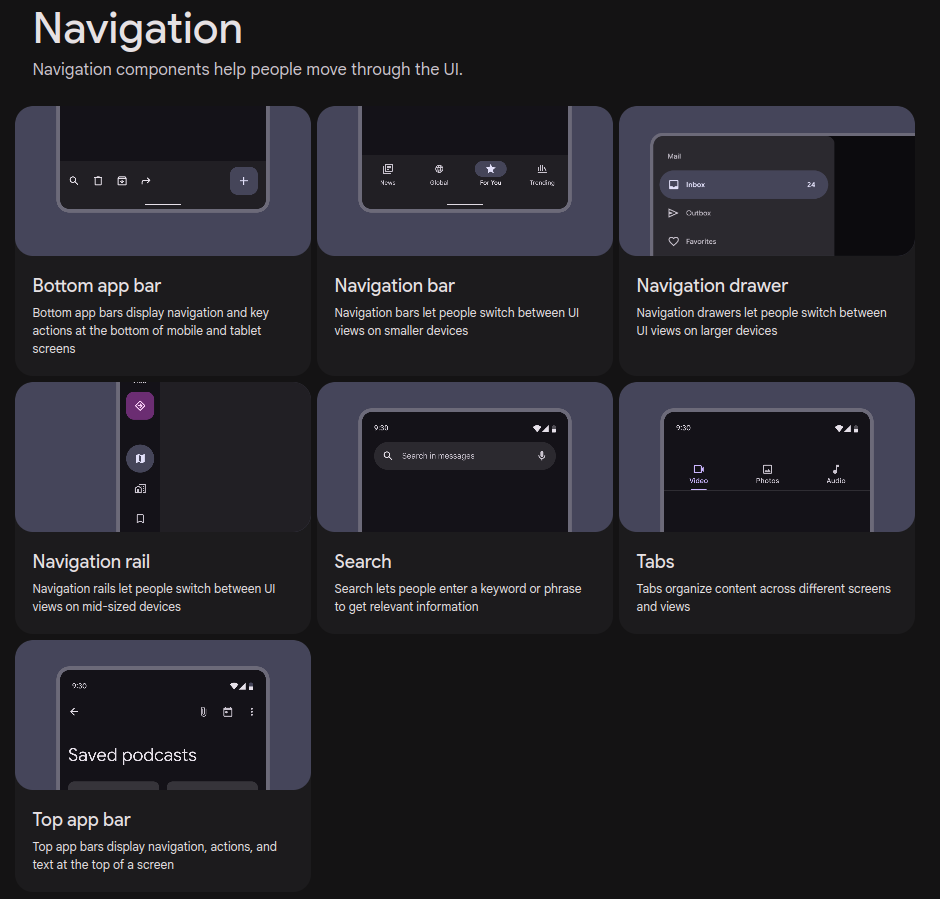
\includegraphics[width=0.7\textwidth]{navigation.png}
        \end{center}
    \end{frame}

    \begin{frame}
        \begin{center}
            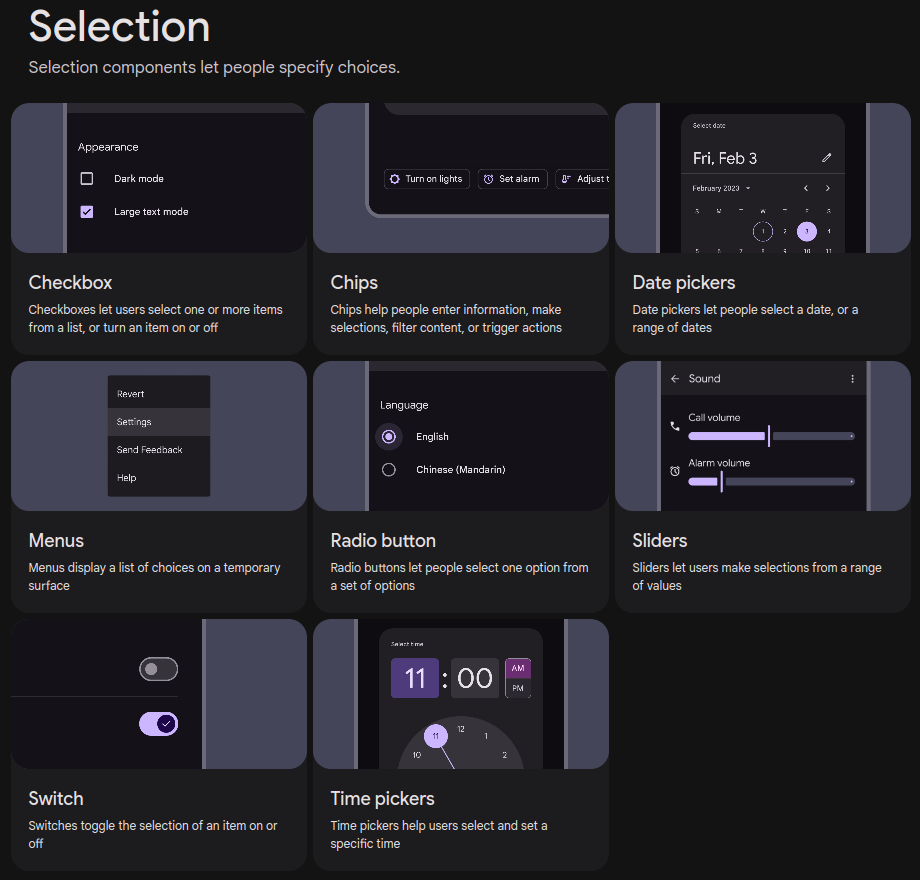
\includegraphics[width=0.7\textwidth]{selection.png}
        \end{center}
    \end{frame}

    \begin{frame}
        \begin{center}
            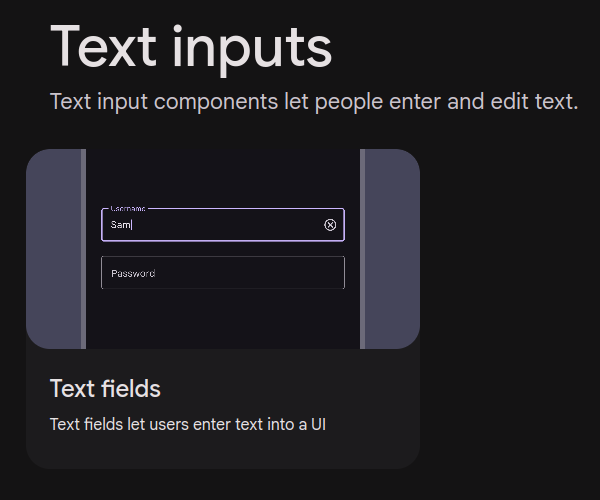
\includegraphics[width=0.7\textwidth]{text-inputs.png}
        \end{center}
    \end{frame}

\end{document}
